\documentclass{article}
\usepackage{tikz}
\usetikzlibrary{positioning, matrix, arrows.meta}
\begin{document}
\begin{itemize}
    \item \textbf{Cruce de un punto (\textit{One Point Crossover} - 1P):}
\begin{center}
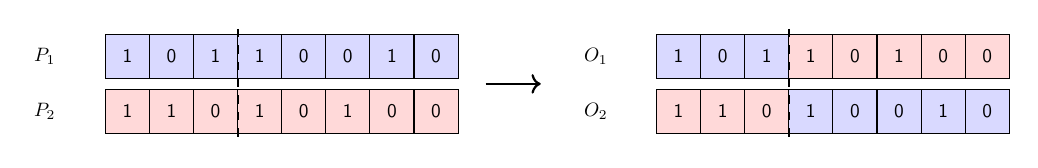
\begin{tikzpicture}[font=\sffamily, scale=0.7, transform shape]
\tikzstyle{bit}=[draw, minimum width=0.8cm, minimum height=0.8cm]
\tikzstyle{p1}=[bit, fill=blue!15]
\tikzstyle{p2}=[bit, fill=red!15]
\node at (-1.5, 1) {$P_1$};
\node[p1] at (0,1) {1}; \node[p1] at (0.8,1) {0}; \node[p1] at (1.6,1) {1}; \node[p1] at (2.4,1) {1}; \node[p1] at (3.2,1) {0}; \node[p1] at (4.0,1) {0}; \node[p1] at (4.8,1) {1}; \node[p1] at (5.6,1) {0};
\node at (-1.5, 0) {$P_2$};
\node[p2] at (0,0) {1}; \node[p2] at (0.8,0) {1}; \node[p2] at (1.6,0) {0}; \node[p2] at (2.4,0) {1}; \node[p2] at (3.2,0) {0}; \node[p2] at (4.0,0) {1}; \node[p2] at (4.8,0) {0}; \node[p2] at (5.6,0) {0};
\draw[->, thick] (6.5, 0.5) -- (7.5, 0.5);
\node at (8.5, 1) {$O_1$};
\node[p1] at (10,1) {1}; \node[p1] at (10.8,1) {0}; \node[p1] at (11.6,1) {1}; \node[p2] at (12.4,1) {1}; \node[p2] at (13.2,1) {0}; \node[p2] at (14.0,1) {1}; \node[p2] at (14.8,1) {0}; \node[p2] at (15.6,1) {0};
\node at (8.5, 0) {$O_2$};
\node[p2] at (10,0) {1}; \node[p2] at (10.8,0) {1}; \node[p2] at (11.6,0) {0}; \node[p1] at (12.4,0) {1}; \node[p1] at (13.2,0) {0}; \node[p1] at (14.0,0) {0}; \node[p1] at (14.8,0) {1}; \node[p1] at (15.6,0) {0};
\draw[dashed, thick] (2.0, 1.5) -- (2.0, -0.5);
\draw[dashed, thick] (12.0, 1.5) -- (12.0, -0.5);
\end{tikzpicture}
\end{center}

    \item \textbf{Cruce de dos puntos (\textit{Two Point Crossover} - 2P):} 
\begin{center}
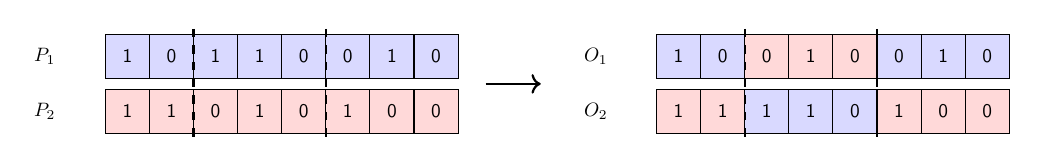
\begin{tikzpicture}[font=\sffamily, scale=0.7, transform shape]
\tikzstyle{bit}=[draw, minimum width=0.8cm, minimum height=0.8cm]
\tikzstyle{p1}=[bit, fill=blue!15]
\tikzstyle{p2}=[bit, fill=red!15]
\node at (-1.5, 1) {$P_1$};
\node[p1] at (0,1) {1}; \node[p1] at (0.8,1) {0}; \node[p1] at (1.6,1) {1}; \node[p1] at (2.4,1) {1}; \node[p1] at (3.2,1) {0}; \node[p1] at (4.0,1) {0}; \node[p1] at (4.8,1) {1}; \node[p1] at (5.6,1) {0};
\node at (-1.5, 0) {$P_2$};
\node[p2] at (0,0) {1}; \node[p2] at (0.8,0) {1}; \node[p2] at (1.6,0) {0}; \node[p2] at (2.4,0) {1}; \node[p2] at (3.2,0) {0}; \node[p2] at (4.0,0) {1}; \node[p2] at (4.8,0) {0}; \node[p2] at (5.6,0) {0};
\draw[->, thick] (6.5, 0.5) -- (7.5, 0.5);
\node at (8.5, 1) {$O_1$};
\node[p1] at (10,1) {1}; \node[p1] at (10.8,1) {0}; \node[p2] at (11.6,1) {0}; \node[p2] at (12.4,1) {1}; \node[p2] at (13.2,1) {0}; \node[p1] at (14.0,1) {0}; \node[p1] at (14.8,1) {1}; \node[p1] at (15.6,1) {0};
\node at (8.5, 0) {$O_2$};
\node[p2] at (10,0) {1}; \node[p2] at (10.8,0) {1}; \node[p1] at (11.6,0) {1}; \node[p1] at (12.4,0) {1}; \node[p1] at (13.2,0) {0}; \node[p2] at (14.0,0) {1}; \node[p2] at (14.8,0) {0}; \node[p2] at (15.6,0) {0};
\draw[dashed, thick] (1.2, 1.5) -- (1.2, -0.5);
\draw[dashed, thick] (3.6, 1.5) -- (3.6, -0.5);
\draw[dashed, thick] (11.2, 1.5) -- (11.2, -0.5);
\draw[dashed, thick] (13.6, 1.5) -- (13.6, -0.5);
\end{tikzpicture}
\end{center}

    \item \textbf{Cruce Uniforme (\textit{Uniform Crossover} - UX):}
\begin{center}
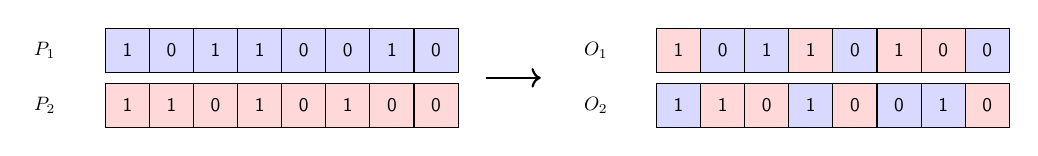
\begin{tikzpicture}[font=\sffamily, scale=0.7, transform shape]
\tikzstyle{bit}=[draw, minimum width=0.8cm, minimum height=0.8cm]
\tikzstyle{p1}=[bit, fill=blue!15]
\tikzstyle{p2}=[bit, fill=red!15]
\node at (-1.5, 1) {$P_1$};
\node[p1] at (0,1) {1}; \node[p1] at (0.8,1) {0}; \node[p1] at (1.6,1) {1}; \node[p1] at (2.4,1) {1}; \node[p1] at (3.2,1) {0}; \node[p1] at (4.0,1) {0}; \node[p1] at (4.8,1) {1}; \node[p1] at (5.6,1) {0};
\node at (-1.5, 0) {$P_2$};
\node[p2] at (0,0) {1}; \node[p2] at (0.8,0) {1}; \node[p2] at (1.6,0) {0}; \node[p2] at (2.4,0) {1}; \node[p2] at (3.2,0) {0}; \node[p2] at (4.0,0) {1}; \node[p2] at (4.8,0) {0}; \node[p2] at (5.6,0) {0};
\draw[->, thick] (6.5, 0.5) -- (7.5, 0.5);
\node at (8.5, 1) {$O_1$};
\node[p2] at (10,1) {1}; \node[p1] at (10.8,1) {0}; \node[p1] at (11.6,1) {1}; \node[p2] at (12.4,1) {1}; \node[p1] at (13.2,1) {0}; \node[p2] at (14.0,1) {1}; \node[p2] at (14.8,1) {0}; \node[p1] at (15.6,1) {0};
\node at (8.5, 0) {$O_2$};
\node[p1] at (10,0) {1}; \node[p2] at (10.8,0) {1}; \node[p2] at (11.6,0) {0}; \node[p1] at (12.4,0) {1}; \node[p2] at (13.2,0) {0}; \node[p1] at (14.0,0) {0}; \node[p1] at (14.8,0) {1}; \node[p2] at (15.6,0) {0};
\end{tikzpicture}
\end{center}

    \item \textbf{Cruce Medio Uniforme (\textit{Half Uniform Crossover} - HUX):}
\begin{center}
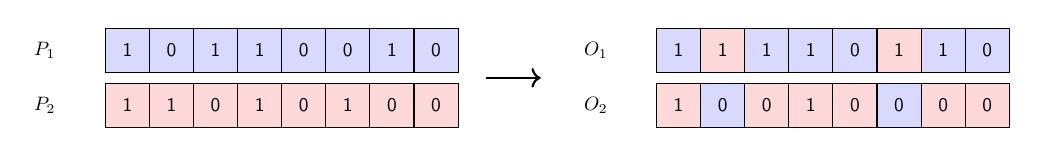
\begin{tikzpicture}[font=\sffamily, scale=0.7, transform shape]
\tikzstyle{bit}=[draw, minimum width=0.8cm, minimum height=0.8cm]
\tikzstyle{p1}=[bit, fill=blue!15]
\tikzstyle{p2}=[bit, fill=red!15]
\node at (-1.5, 1) {$P_1$};
\node[p1] at (0,1) {1}; \node[p1] at (0.8,1) {0}; \node[p1] at (1.6,1) {1}; \node[p1] at (2.4,1) {1}; \node[p1] at (3.2,1) {0}; \node[p1] at (4.0,1) {0}; \node[p1] at (4.8,1) {1}; \node[p1] at (5.6,1) {0};
\node at (-1.5, 0) {$P_2$};
\node[p2] at (0,0) {1}; \node[p2] at (0.8,0) {1}; \node[p2] at (1.6,0) {0}; \node[p2] at (2.4,0) {1}; \node[p2] at (3.2,0) {0}; \node[p2] at (4.0,0) {1}; \node[p2] at (4.8,0) {0}; \node[p2] at (5.6,0) {0};
\draw[->, thick] (6.5, 0.5) -- (7.5, 0.5);
\node at (8.5, 1) {$O_1$};
\node[p1] at (10,1) {1}; \node[p2] at (10.8,1) {1}; \node[p1] at (11.6,1) {1}; \node[p1] at (12.4,1) {1}; \node[p1] at (13.2,1) {0}; \node[p2] at (14.0,1) {1}; \node[p1] at (14.8,1) {1}; \node[p1] at (15.6,1) {0};
\node at (8.5, 0) {$O_2$};
\node[p2] at (10,0) {1}; \node[p1] at (10.8,0) {0}; \node[p2] at (11.6,0) {0}; \node[p2] at (12.4,0) {1}; \node[p2] at (13.2,0) {0}; \node[p1] at (14.0,0) {0}; \node[p2] at (14.8,0) {0}; \node[p2] at (15.6,0) {0};
\end{tikzpicture}
\end{center}
\end{itemize}
\end{document}
